\documentclass[]{mattcv}

\usepackage{xcolor}
% flat ui colors
\definecolor{alizarin}{RGB}{231,76,60}
\definecolor{belizehole}{RGB}{41,128,185}
\definecolor{carrot}{RGB}{230,126,34}
\definecolor{emerald}{RGB}{46,204,113}
\definecolor{nephritis}{RGB}{39,174,96}
\definecolor{peterriver}{RGB}{52,152,220}
\definecolor{turquoise}{RGB}{26,188,156}
\definecolor{wetasphalt}{RGB}{52,73,94}

\usepackage{bbding}
\usepackage{dirtytalk}
\usepackage{everypage}
\usepackage[colorlinks=true, urlcolor=wetasphalt]{hyperref}
\usepackage[alpine, misc]{ifsym}
\usepackage{pgf-pie}
\usepackage{tikz}

\AddEverypageHook{%
    \cvheader
        {Mateusz} % first name(s)
        {Jemielity} % last name
        {40} % names fontsize
        {Software Engineer} % job title
        {20.3} % job title fontsize
        {matt.eps} % eps picture filepath
    }

\begin{document}

    \cvsection{contact}{wetasphalt}{%
        \begin{center}
            \FilledHut\hspace{2mm}Warszawa, Polska\hspace{1cm}\PhoneHandset\hspace{2mm}+48000000000\hspace{1cm}\Letter\hspace{2mm}...@gmail.com\\
            \href{https://google.com/+MateuszJemielity/about}{Google+}\hspace{1cm}\href{https://github.com/Matthew-Jemielity}{Github}
        \end{center}
    }
    \cvsection{about}{carrot}{%
        \say{When you solve a puzzle the world makes sense and everything feels right.} (House MD)
        \par
        Thus I solve puzzles. Mainly from domains of computer science and software engineering. The more I know, the more interesting puzzles I can tackle. I wand to know (and solve) everything, in time.
        \par
        I'm an enthusiastic programmer and C is my language of choice, though I don't shy away from different ones. During my career I went from debugging to writing drivers, from making Linux kernel boot on new devices, to contributing to ambitious userland projects. I'm looking for an opportunity to expand my knowledge of the field and a chance to polish my skills.
    }
    \cvsection{experience}{emerald}{%
        \cvtimeline{\textbf{Software Engineer}, Samsung Electronics Poland R\&D Center}{nephritis}{2013}{2015}{%
            \begin{itemize}
                \item contributed to internal projects ranging from performance benchmarking to structured light 3D scanning
                \item investigated performance- and power consumption-related issues in ARM-based embedded systems
                \item developed Linux kernel drivers and userland applications for Android OS and GNU/Linux
                \item worked in C, C++, Java and Python
            \end{itemize}
        }
        \cvtimeline{\textbf{Junior Software Engineer}, Samsung Electronics Poland R\&D Center}{nephritis}{2009}{2013}{%
            \begin{itemize}
                \item was responsible for debugging and porting exisitng projects to new devices
                \item worked as a part of international team, recognized as top contributor
                \item handled bringup of Linux kernel on new ARM-based hardware
                \item implemented new features across proprietary bootloader, L4-based RTOS, Android OS
                \item worked with ARM-based embeded systems, mainly in C
            \end{itemize}
        }
    }
    \cvsection{education}{peterriver}{%
        \cvtimeline{\textbf{Informatics}, University of Gdańsk}{belizehole}{2004}{2009}{%
            \begin{itemize}
                \item uniform magister-level courses (MSc)
                \item \href{http://arch.ug.edu.pl/pl/najlepsi/index.php?strona=student&id_stud=526&lang=en}{best student 2008/2009}
                \item thesis title: \say{Turing Machine in Conway's Game of Life}
            \end{itemize}
        }
    }
    \cvsection{skills}{alizarin}{%
        \begin{center}
            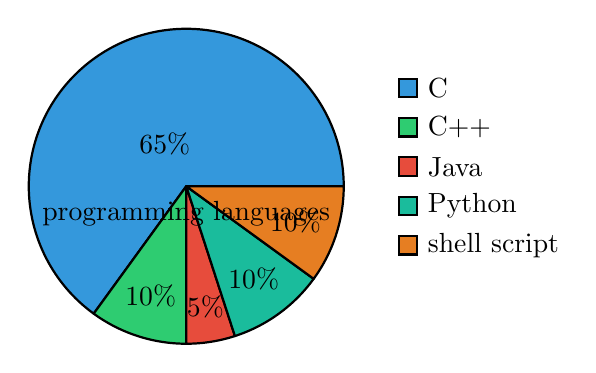
\begin{tikzpicture}
                \pie[
                    color={peterriver, emerald, alizarin, turquoise, carrot},
                    radius=2,
                    text=legend
                ]{65/C, 10/C++, 5/Java, 10/Python, 10/shell script}
                \node [below=2, align=flush center] {programming languages};
            \end{tikzpicture}
            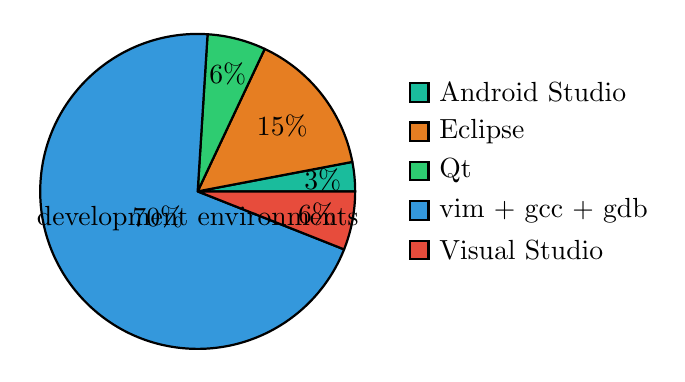
\begin{tikzpicture}
                \pie[
                    color={turquoise, carrot, emerald, peterriver, alizarin},
                    radius=2,
                    text=legend
                ]{3/Android Studio, 15/Eclipse, 6/Qt, 70/vim + gcc + gdb, 6/Visual Studio}
                \node [below=2, align=flush center] {development environments};
            \end{tikzpicture}
        \end{center}
    }

\end{document}

